
%(BEGIN_QUESTION)
% Copyright 2010, Tony R. Kuphaldt, released under the Creative Commons Attribution License (v 1.0)
% This means you may do almost anything with this work of mine, so long as you give me proper credit

Suppose an electric actuator is used to lift a large concrete gate in an irrigation water flow control facility.  The gate effectively acts as a control valve for water flowing through an open irrigation channel, and a powerful winch is necessary to control its position:

$$\includegraphics[width=15.5cm]{i00584x01.eps}$$

The winch drum measures 20 inches in diameter, and the concrete gate weighs 12,740 pounds.  Calculate the torque required at the drum to lift the gate, and also the torque required by the electric motor given a gearbox speed-reduction ratio of 1200:1.

Assuming the electric motor powering this speed-reducing gearbox spins at 1720 RPM (at full load), calculate the vertical lifting speed of the gate in feet per minute.  Finally, calculate the horsepower output of the electric motor lifting this much weight (12,740 pounds) at this vertical speed.

\vskip 20pt \vbox{\hrule \hbox{\strut \vrule{} {\bf Suggestions for Socratic discussion} \vrule} \hrule}

\begin{itemize}
\item{} Like all ``story problems'' involving mathematical calculation, the most important aspect of your answer is {\it how} you arrived at it, not the numerical value(s) of your answer.  Explain how you were able to set up the proper equations to solve for drum torque, motor torque, lifting speed, and motor output power.
\item{} A useful problem-solving technique is to sketch a simple diagram of the system you are asked to analyze.  This is useful even when you already have some graphical representation of the problem given to you, as a simple sketch often reduces the complexity of the problem so that you can solve it more easily.  Draw your own sketch showing how the given information in this problem inter-relates, and use this sketch to explain your solution.
\end{itemize}

\underbar{file i00584}
%(END_QUESTION)





%(BEGIN_ANSWER)

\noindent
{\bf Partial answer:}

\vskip 10pt

$\tau_{motor}$ = 8.8472 lb-ft

\vskip 10pt

Motor output = 2.897 horsepower

%(END_ANSWER)





%(BEGIN_NOTES)

Torque on the winch drum is the product of drum radius and applied weight.  In this case, the radius is 10 inches (0.8333 ft) which when multiplied by 12740 pounds gives us 10616.7 lb-ft of torque at the drum.  Since the motor spins the drum through a 1200:1 gear reduction, the motor need only apply 1/1200 of this torque, or 8.8472 lb-ft of torque at the motor shaft.

\vskip 10pt

The motor's speed of 1720 RPM will be reduced by the gear set by a ratio of 1200:1 to a much slower drum speed of 1.4333 RPM.  Since each rotation of the drum equates to one circumference worth of linear gate motion, we may multiply the rotational speed of 1.4333 RPM by the drum's circumference ($C = \pi d = 20 \pi = 62.83$ inches) to get a vertical lifting speed of 90.06 inches per minute or 7.505 feet per minute.

\vskip 10pt

Power is work done per unit time.  The amount of work done by this motor and winch drum per minute of time is equal to the weight of the gate multiplied by the displacement (lift) per minute, or 12740 lb times 7.505 ft/min.  This equals 95612.6 ft-lb of work per minute of time.  One horsepower is equal to 550 ft-lb per second of time, so this motor is outputting 2.897 HP.

%INDEX% Physics, energy, work, power: calculating work and power
%INDEX% Physics, torque: calculation problem

%(END_NOTES)

